\documentclass[12pt, a4paper]{article}
\setcounter{tocdepth}{2}
\usepackage{graphicx} % Required for inserting images
\usepackage[parfill]{parskip} % Removes indent from new paragraphs
\usepackage{amsmath, amssymb, amsfonts}
\usepackage[colorlinks = true,
			citecolor  = blue,
            linkcolor = black]{hyperref}
\usepackage[font={small,it}]{caption}
\usepackage[labelfont=bf]{caption}

\usepackage[natbibapa]{apacite}
\bibliographystyle{apacite}
% \usepackage[longnamesfirst,authoryear, round]{natbib}
% \bibliographystyle{unsrtnat}

\usepackage[
top    = 1.0in,
bottom = 1.2in,
left   = 1.0in,
right  = 1.0in]{geometry}
\linespread{1.5}

\title{Comparison of MCMC algorithms in Stochastic Volatility Models}
\author{Benjamin Wee}
\date{October 2023}

\begin{document}

\maketitle 

\begin{abstract}
    This research compares the computational methods used to estimate Bayesian stochastic volatility models. The estimation strategies outlined in the stochastic volatility literature and Hamiltoninan Monte Carlo are assesssed in their ability to sample from the model's posterior distribution. Specifically, Simulation Based Calibration (SBC) is used to check whether these MCMC algorithm are returning efficient and well calibrated posterior estimates. Key metrics of interest are the effective sample size to check the efficiency of the algorithm and tests of uniformity to assess the calibration of the posteriors. This will determine which method is better at estimating stochastic volatility models based on the efficiency and accuracy of the sampling strategy. Results reveal that Hamiltonian Monte Carlo provides more efficient and calibrated posterior estimates conditional on the non centered paramterisation of the stochastic volatility model. 
\end{abstract}

\newpage

\tableofcontents{\protect\newpage}

\section{Introduction}
    The stochastic volatility model is used in financial econometrics to model the behaviour of financial instruments. It explicitly treats the variance as a latent random variable. These are typically expressed as non linear Gaussian state space models and are difficult to estimate using classical methods. The likelihood is unavailable in closed form and there are at least as many variables as data points. Bayesian approaches to estimating these models rely on  Markov Chain Monte Carlo (MCMC) techniques to sample from the target joint posterior of these high dimensional latent parameter spaces. 

    \citet{kim1998stochastic} propose a method for sampling this model using a combination of Kalman Filters, Gibbs sampler, and Metropolis Hastings over 20 years ago.  Since then, there have been many advances in statistical computing to estimate complex, high dimensional Bayesian models. In particular, the recent availability of Hamiltonian Monte Carlo, a variant of the Metropolis Hastings algorithm, is an advancement of MCMC for efficient sampling of complex probabilistic models. The adoption of such new techniques have been made widely available through the development of various open source libraries such as the Stan programming language \citep{stan} and the PyMC library \citep{pymc2023}. Other algorithms have also improved the speed of estimating high dimensional models using approximations of the posterior such as integrated nested Laplace approximation \citep{rue2009approximate}.

    These conceptually and practically different techniques to estimate complex models did not exist 20 years ago (or perhaps more accurately, were not easily accessible or implemented 20 years ago). As the development of new algorithms rapidly increase, so does the need to develop new methods to assess their output. Developments in our statistical workfow are required to test new algorithms as well as compare computational strategies used to estimate increasingly complex models.

    This research conducts a simulation study to assess the algorithms used to estimate stochastic volatility models. The first algorithm replicates Kim Sherphard and Chib's (KSC) Gaussian mixture approximation which is applied on a transformed stochastic volatility model with a log chi squared error distribution. Their sampling method uses the aforementioned Kalman Filter estimating the latent states, conjugate posterior distributions and the Metropolis Hastings algorithm. The second algorithm is the Hamiltonian Monte Carlo (HMC) algorithm as implemented in the Stan programming language. The objective is to analyse the efficiency of the sampling approach and their ability to return calibrated posterior estimates. 

    Comparisons of these algorithms are conducted by Simulation Based Calibration \citep{talts2018validating}. Parameters are drawn from the prior distribution and used to create datasets from the generative (stochastic volatility) model which are sampled using a MCMC method. Repeating this process multiple times gives insight to how well the sampling approach can estimate the true parameters governing the data generating process on average. The key diagnostic metrics are the effective sample size to measure the efficiency of the algorithm and visual tests of uniform rank statistics to assess calibration of the posterior estimates. 

    Additionally, two different parametiersations of the stochastic volatility model are considered for each sampling method. These are described as either 'centred' or 'non-centred' in location. An algorithm may be sensitive to different parameterisations of the same model which may impact MCMC efficiency as described in \citet{strickland2008parameterisation}. The key contribution of this research is to use simulations to assess whether a MCMC algorithm can return calibrated posterior estimates as well as the efficiency under the different parametiersations.

    This paper is structured as follows. Section 2 provides the context around this research, namely the stochastic volatility model examined and the limitations of single simulation studies and MCMC convergence diagnostics. Section 3 describes the simulation design and diagnostic metrics. Section 4 details the sampling approaches. Section 5 discusses the results and limitations. Finally, section 6 concludes and provides points for further reserach.

\section{Resarch Context}

\subsection{Stochastic Volatility}
    The model of interest is the discrete time, univariate stochastic volatility model estimated by \citet{kim1998stochastic} using Bayesian methods. $y_t$ is the mean corrected returns of some asset for equally spaced intervals t. $\beta$ is a constant scaling factor which is also defined as $exp(\mu / 2)$ representing instantaneous volatility. $h_t$ is log volatility, where $h_1$ is a draw from a stationary distribution and the state equation $h_{t+1}$ follows a stationary process governed by the autoregressive parameter $\phi$ such that $|\phi|<1$. This autoregressive parameter represents the persistence or "stickiness" of log volatility and the dispersion parameter $\sigma_{\eta}$ is the constant variance of the states. $\epsilon_t$ and $\eta_t$ are standard normal white noise shocks and are uncorrelated with each other. 

    $$
    \begin{aligned}
    y_t =& \space \beta exp(h_t/2) \epsilon_t \\
    h_{t+1} =& \space \mu +\phi(h_t - \mu) + \sigma_{\eta} \eta_t  \\
    h_1 \sim& \space normal\left(\mu, \frac{\sigma_{\eta}^2}{1-\phi^2}\right) \\
    \end{aligned}
    $$


    $$
    \begin{aligned}
    \epsilon_t \sim& \space normal(0,1) \\
    \delta_t \sim& \space normal(0,1)
    \end{aligned}
    $$

    Setting $\beta=1$, the model can be expressed more succinctly as:

    $$
    \begin{aligned}
    y_t \sim& \space normal(0, exp(h_t/2)) \\ 
    h_1 \sim& \space normal \left(\mu, \frac{\sigma_{\eta}^2}{1-\phi^2}\right) \\
    h_{t+1} \sim& \space normal(\mu +\phi(h_t - \mu) , \sigma_{\eta}^2), \space\space t\neq 1\\ 
    \end{aligned}
    $$

    Priors for the static parameters are defined below with conjugate priors on $\mu$ and $\sigma^2$:

    $$
    \begin{aligned}
    \mu \sim& \space normal(0, 10^2) \\
    \sigma_{\eta}^2 \sim& \space IG(5/2, (0.01\times 5) / 2) \\
    \phi^{\ast} \sim& \space beta(20, 1.5) \\
    \phi &=  2\phi^{\ast} - 1
    \end{aligned}
    $$

    The prior on $\phi$ is a "stretched" beta distribution. This is a beta distribution (as defined on the parameter $\phi^*$) which has been transformed to have support (-1, 1).


\subsection{Diagnostic limitations on real data}
    The stochastic volatility model can be estimated using a variety of sampling strategies and MCMC algorithms. Convergence metrics are often used to check the performance of the MCMC chains, such as the effective sample size and the $\hat{R}$. These diagnostics provide evidence on whether an MCMC has failed to converge onto the target posterior distribution.

    Convergence diagnostics are useful for identifying when Bayesian computation fail on real data. However, confounding issues may arise when attempting to diagnose the cause of computational problems. Real data is generated from an unknown data generating process. That is, the true parameter or model is unobservable. Therefore, failed diagnostic checks could arise from either inocrrect model specification or issues in the sampling algorithm or both.

    Furthermore, different sampling strategies and MCMC tools could provide different posterior estimates for the same model. Assuming no issues in computation, these diagnostic measures do not provide any evidence to which estimate is closer to the truth.

    To illustrate this problem, the stochastic volatility model is estimated with two different MCMC algorithms on real data. The data are the de-meaned log returns of the 2023 January-September S\&P 500 Index. Below are the marginal posterior estimates for the static parameters $\mu$, $\phi$ and $\sigma^2$ and corresponding summary statistics.

    \begin{figure}[h]
        \centering
        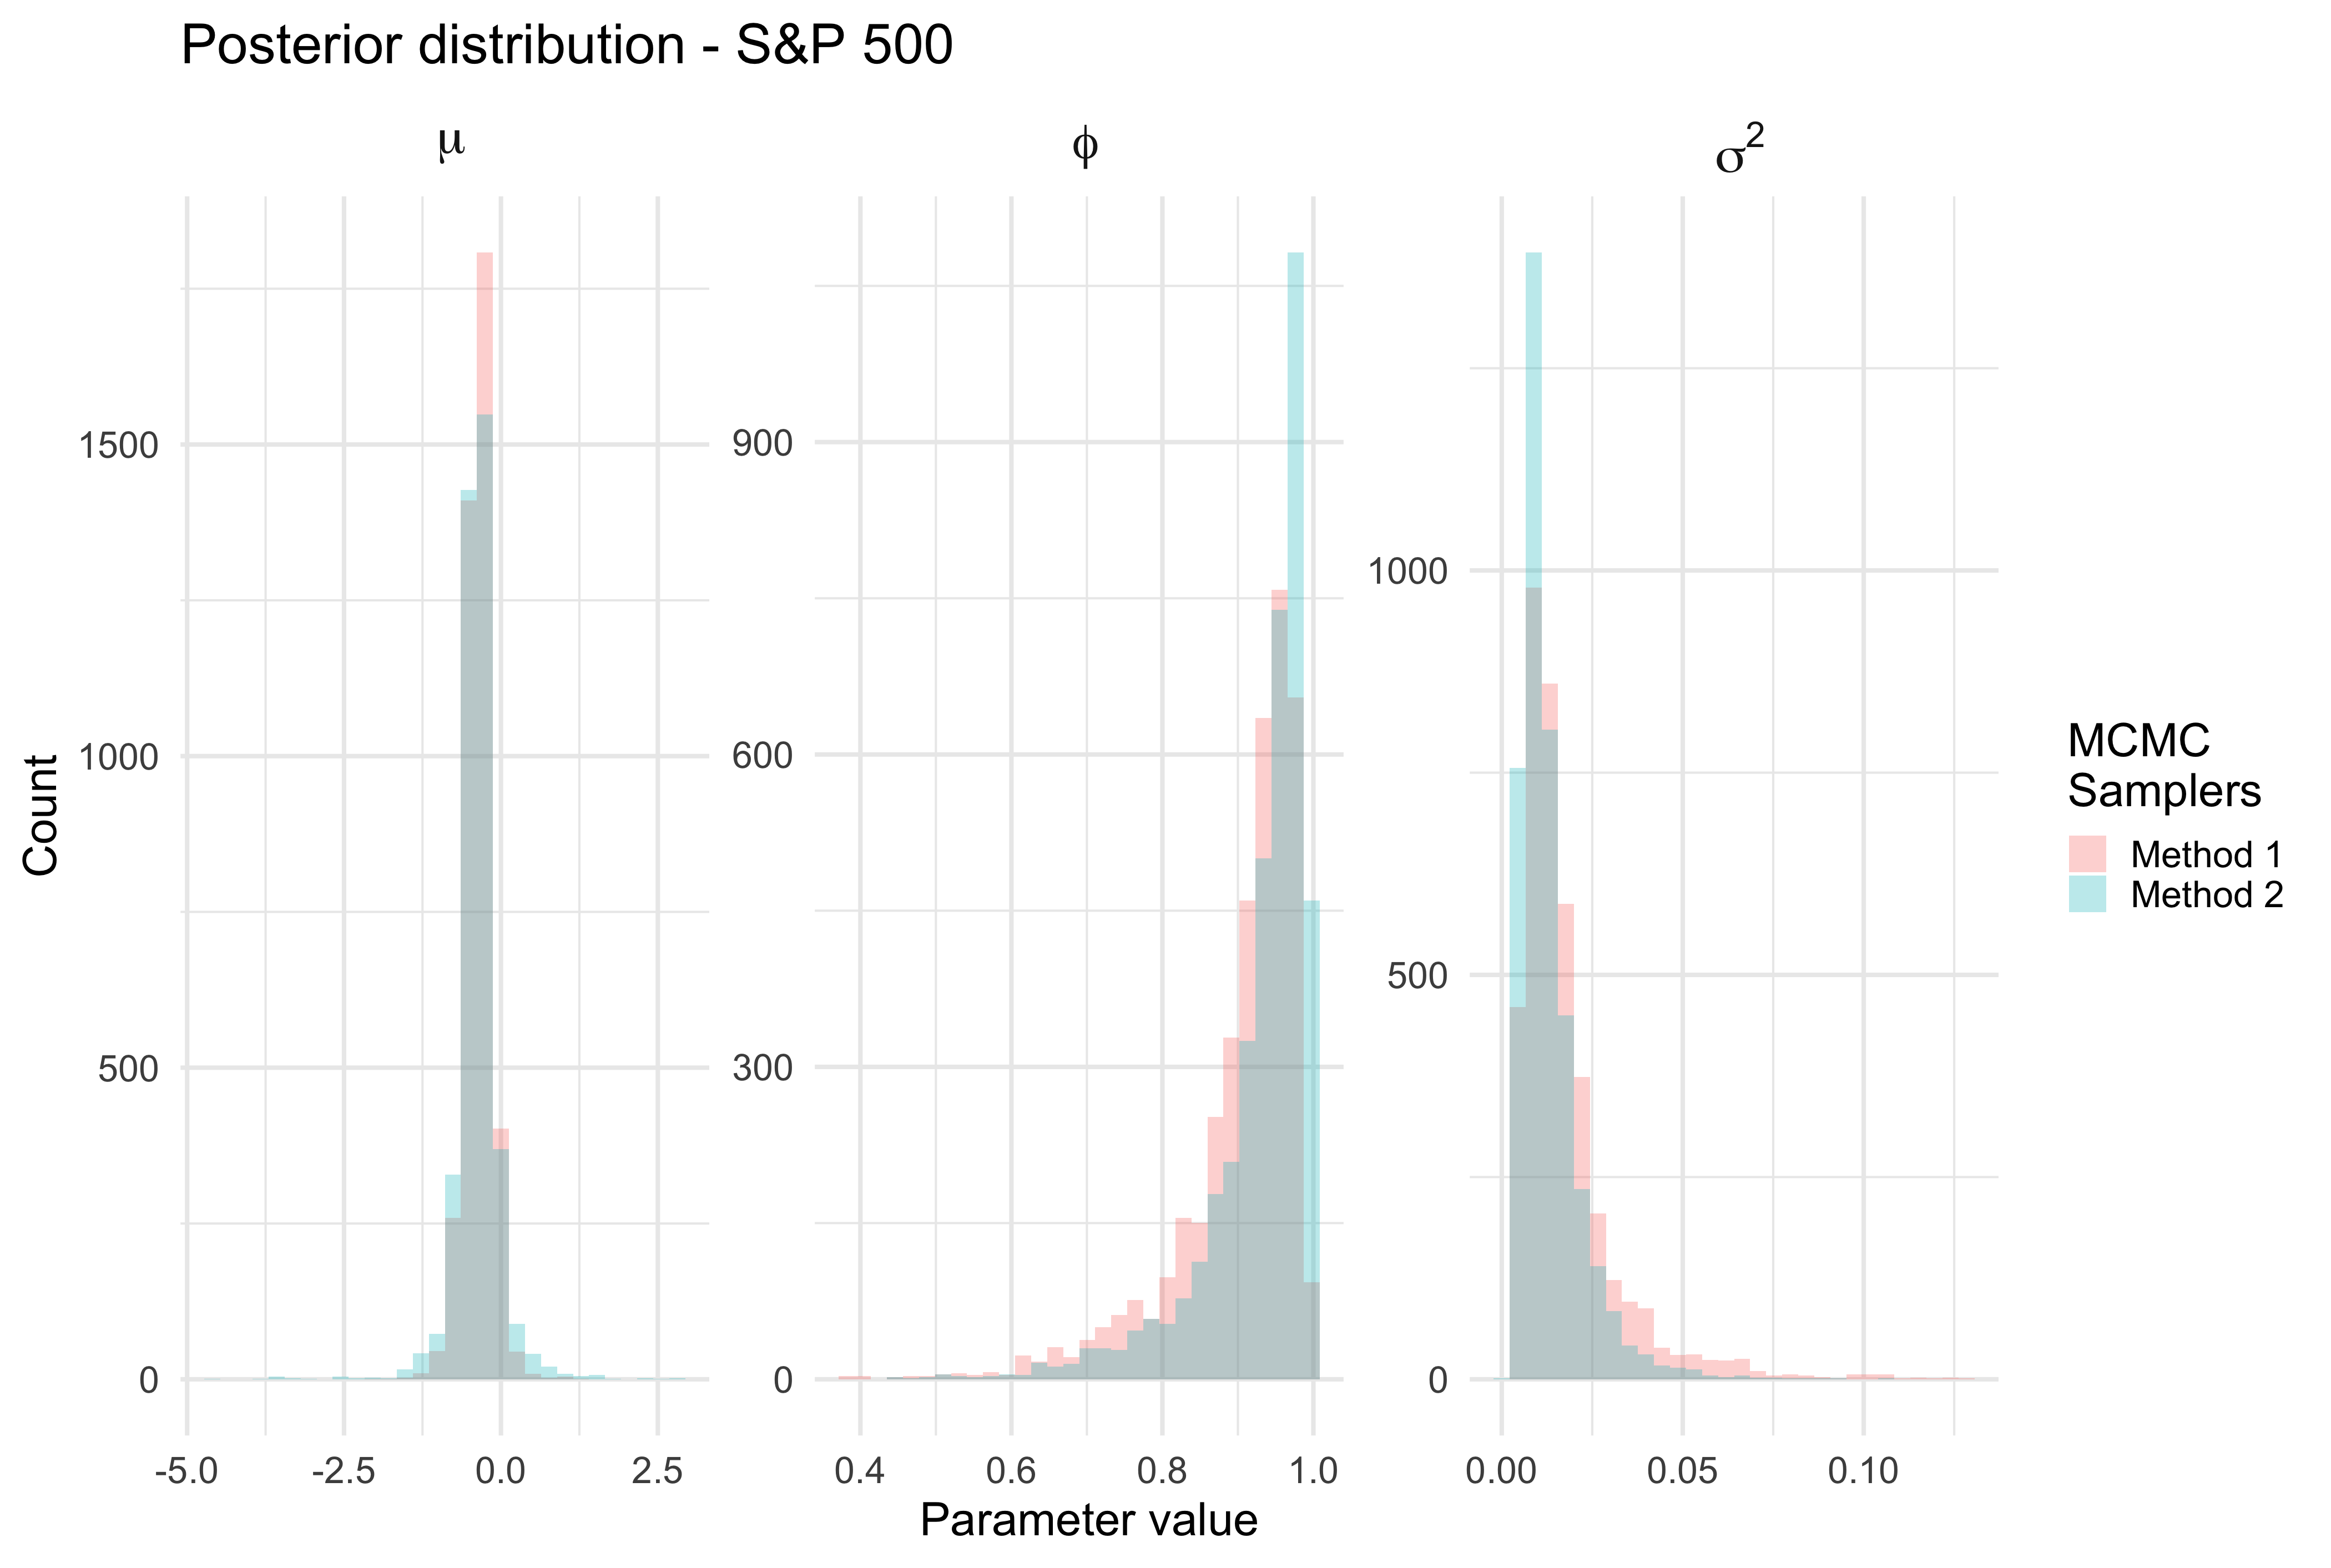
\includegraphics[scale=0.1]{motivating_example/real_data_ex.png}
        \caption{Posterior samples from two MCMC algorithms using S\&P 500 data}
    \end{figure}

    These estimates show the marginal posteriors of each parameter sharing similar shapes. $\phi$  has a fatter left tail for and $\sigma^2$ has heavier right tails for sampling method 1 (SM1). Furthermore, SM2 has higher peaks at their mode relative to SM1 with a tighter spread. Based on this information alone, there is no certainty in whether SM1 or SM2 is has a more correct estimate conditional on data and model. There are other methods for model or algorithmic selection in this context (for example, out of sample predictive performance), but for parameter estimation it is unclear which one should be selected. 

\subsection{Diagnostic limitations on a single simulation}
    Diagnosing computational problems on real data is difficult due to confounding factors. A strategy around this is to evaluate a model and algorithm on simulated data. One approach is to simulate data from the proposed model using known parameters. Then, fit the model on the simulated data and see if the model can recover the true parameters. This gives us the benefit of defining the true parameters of the data generating process to be estimated. If the model and algorithm cannot adequately capture the true parameter, then we cannot be confident that it will provide reliable estimates on real data.

    Furthermore, as discussed in \citet{gelman2020bayesian}, fitting models on simulated data is the only way we can check inference on latent variables. This is critical in Stochastic Volatility since the underlying framework is a state space model with latent log volatility parameters. Latent variables are unobserved in real data and are only estimated in the context of the model. Simulation gives control over the data generating process which reveals what the model can infer about the latent variables. 

    Simulations enable us to check whether our models and algorithms can estimate the true data generating process, however, there are limitations to what can be learned from a single simulation. There is always a small probability that the true parameter is in the tails of any estimated posterior distribution. Or put differently, there is a 1\% chance the true parameter or any random draw exists outside a 99\% credible interval. \cite{talts2018validating} make the point that a single simulation does not provide sufficient information about the inference made by an algorithm. As discussed in their paper, a single simulation may conclude "that an incorrectly coded analysis worked as desired, while a correctly coded analysis failed". 

    The below results are from a single simulation where data is generated and sampled from the stochastic volatility model with known parameters.

    \begin{figure}[h]
        \centering
        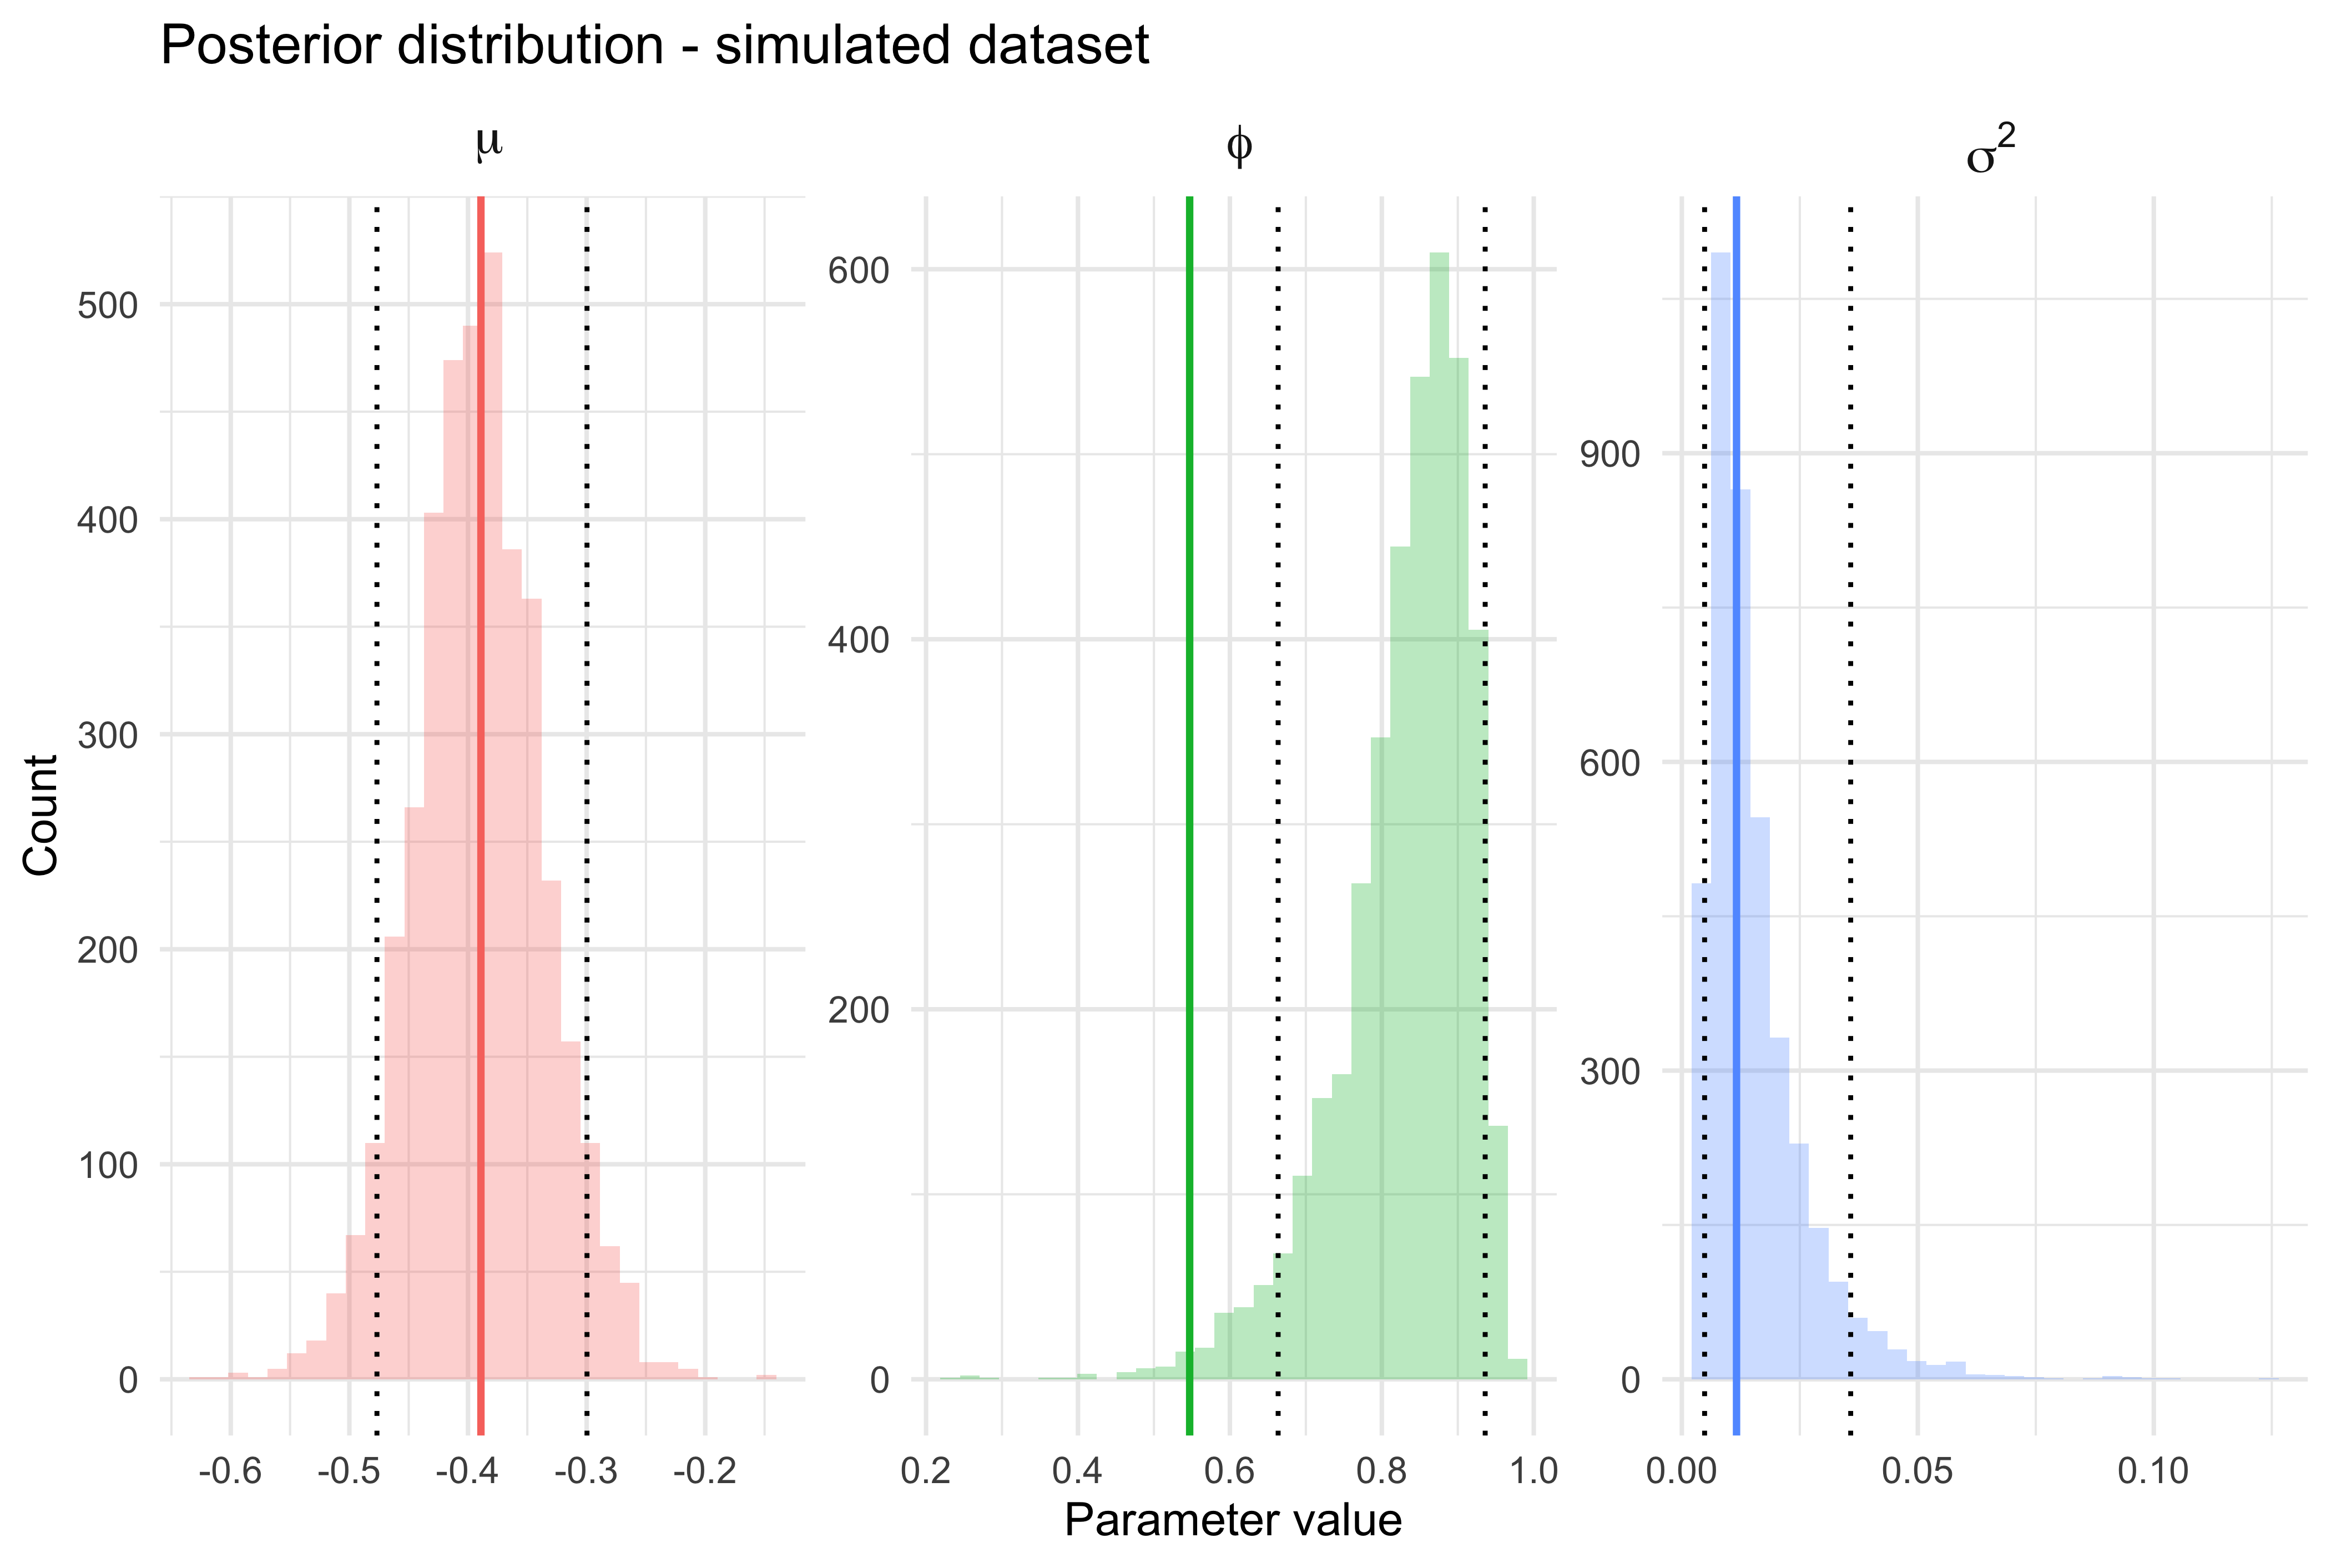
\includegraphics[scale=0.1]{motivating_example/single_sim.png}
        \caption{Posterior samples from known data genearting process. Vertical solid line represents true parameter and dotted lines are 95\% credible intervals around the mean}
    \end{figure}

    The 95\% credible intervals for $\mu$ and $\sigma^2$ cover the true parameter. The true parameter for $\phi$ however, is in the tails and outside the interval. Such an analysis may incorrectly conclude that the model fails to adequatly estimate the $\phi$ parameter. However, it may be the case that the posterior distribution is correctly calculated using this algorithm and the results may be due to the features of this specific simulated dataset.

\subsection{Research Goal}
    The objective of this research is to design a simulation study to evaluate the calibration of algorithms used to sample Stochastic Volatility models. Indeed, there are limitations to evaluating MCMC algorithms based on fits to real data and single simulations. To check the calibration of an algorithm, simulations over multiple "true parameters" are required. This methodology is discussed in the next section. 

    Additionally, two sampling strategies will be assessed using the proposed simulation design as well as the performance of the samplers under different parameterisations of the stochastic volatility model. Not only will the calibration of any one algorithm be assessed, but also compared across sampling strategies to determine which MCMC approach is most suitable for estimating this model. 

\section{Methodology}

    \subsection{Simulation Design}
        Simulation Based Calibration (SBC) checks the calibration of posterior estimates generated by MCMC algorithms. SBC is conducted by comparing the distribution of rank statistics to the discrete uniform distribution which arises when an algorithm is correctly calibrated. The procedure starts by taking draws from the prior distribution and creating datasets implied by each draw. Rank statistics are then calculated on the posterior samples conditional on the simulated data. 

        To illustrate this procedure, let $\theta$ be a parameter and $y$ represent the dataset. Start with a single draw from the prior distribution:
        
        $$
        \begin{aligned}
        \theta^{sim} \sim \pi(\theta)
        \end{aligned}
        $$

        Generate a dataset given by the prior draw.

        $$
        \begin{aligned}
        y^{sim} \sim \pi (y|\theta^{sim})
        \end{aligned}
        $$

        Then take draws from the posterior distribution generated by a MCMC algorithm or estimation strategy (Hamiltonian Monte Carlo or KSC) conditional on this dataset.

        $$
        \begin{aligned}
        \{\theta_1,\dots , \theta_{L}\} \sim \pi (\theta | y^{sim})
        \end{aligned}
        $$

        A key result is that the posterior sample $\{\theta_1,\dots , \theta_{L}\}$ will share the same distribution as the prior samples $\theta^{sim}$. This is implied by the following expression:

        $$
        \begin{aligned}
        \pi(\theta) &= \int \pi(\theta|y^{sim}) \pi(y^{sim}|\theta^{sim}) \pi(\theta^{sim})dy^{sim} d\theta^{sim} \\
        &= \int \pi(\theta|y^{sim}) \pi(y^{sim},\theta^{sim}) dy^{sim} d\theta^{sim}
        \end{aligned}
        $$

        That is, the posterior averaged over the joint distribution follows the same distribution as the prior. The procedure of generating posterior samples implicitly performs this integral since the expression on the right of the integral is proportional to the prior density. Therefore, any deviation of the posterior samples from the prior distribution suggests that the sampling methodology is not producing the correct posteriors.

        If the posterior samples follows the prior distribution, the rank statistic for a given parameter follows a discrete uniform distribution\footnote{Proof of this result in \citet{talts2018validating}.}. The rank statistic is defined as:

        $$
        \begin{aligned}
        r = rank(\{\theta_1,\dots , \theta_{L}\}, \theta^{sim}) = \sum_{l=1}^{L}1[\theta_{l} < \theta^{sim}]
        \end{aligned}
        $$

        This completes one iteration of SBC. To complete the algorithm, multiple iterations are run and the rank statistics are calculated for each parameter. The resulting rank statistics are compared to the discrete uniform distribution to determine if any problematic features exist.

        If the computation is well calibrated and the rank statistics follow a discrete uniform distribution, then the posterior credible intervals have sufficient coverage. That is, one way to describe calibration is: for any percentage interval selected over the posterior samples (for example 90\%) then there is a 90\% chance that $\theta^{sim}$ falls within this interval. Another way of saying this is a Bayesian analysis is well calibrated if a 90\% credible interval contains the true parameter in 90\% of the SBC iterations. 

    \subsection{Evaluation Metrics}
        The key metrics and diagnostics to compare the performance of these methods are the effective sample size (ESS), rank statistics, and chi-squared test statistics. 
        
        \subsubsection{Effective sample size}
            ESS measures the efficiency of the MCMC sampler. It calculates the number of effectively independent draws from the posterior draws generated by a Markov chain. A poor ESS can arise from high autocorrelation in the Markov chain which leads to highly dependent samples. An efficient MCMC algorithm takes less resources (for example, time and number of draws) to get a representative sample of the target distribution. If a MCMC algorithm possesses higher ESS for the majority of its parameters (relative to another strategy), then there is evidence that this method is a more efficient sampler. 
    
        \subsubsection{Rank statistics and chi squared statistics}
            Rank statistics as described in the SBC section are used to evaluate the calibration of a posterior. Histograms will be used to evaluate the distribution of rank statistics. If a posterior is well calibrated then it is expected that the histogram is uniform.
    
            A drawback of this approach is there are more parameters than data points in this model. An alternative to visually checking for uniformity of all the parameters is to calculate the chi squared statistics for the counts in each histogram bin. Let $b_j$ be the number of counts and $e_j$ the expected count in bin $j$. Then the chi squared statistic is given by:
            
            $$
            \begin{aligned}
            \chi^2 = \sum_{j=1}^J \frac{(b_{j} - e_{j})^2}{e_j}
            \end{aligned}
            $$
            
            A perfectly discrete uniform distribution will return a $\chi^2$ statistic of zero. That is, the number of rank statistics in each bin is equal to the expected number conditional on the number of bins and observations. Instead of performing multiple hypothesis tests for each parameter, the distribution of $\chi^2$ statistics is compared across all parameters and simulations. This will give a high level summary of calibration and overall performance of the algorithms.        

\section{MCMC Strategies}

    \subsection{Sampling method 1}
        (KSC) sample the posteriors of the stochastic volatility model using a mix of conjugate posterior distributions, Metropolis Hastings and the Kalman Filter and smoother\footnote{In this research the exact software to apply the simulation smoother is unavailable, so a more recent simulation smoother is used which is based on the software written by the same author.} \citep{dejong1995}.

        The standard Kalman Filter and smoother is used to compute the posterior distribution over the latent states. This requires the state and measurement equations to be linear and conditionally Gaussian. Since the relationship between $y_t$ and $h_t$ in the measurement equation is not linear, a transformation is applied by squaring and taking the log of $y_t$.

        $$
        \begin{aligned}
        y_t^{*} &= log(y_t^2) \\ 
        &= log((\epsilon_t exp(h_t/2))^2) \\
        &=  log(exp(h_t)) + log(\epsilon_t^2) \\
        &= h_t + log(\epsilon_t^2)  \\
        &= h_t + z_t \\
        \end{aligned}
        $$

        Where $z_t = log(\epsilon_t^2)$ follows a log chi-squared distribution with mean -1.2704 and variance 4.93. The relationship between $y_t$ and $h_t$ is now linear; however, the error is not Gaussian. Since it is not simple to sample from this parameterisation of the model, KSC use a mixture of Gaussians to **approximate** the first 4 moments of the log chi squared distribution. This is defined by:

        $$
        \begin{aligned}
        f(z_t) = \sum_{i=1}^{K} q_if_N(z_i|m_i-1.2704, \nu_i^2)
        \end{aligned}
        $$

        Where K is the mixture of normal densities $f_N$, component probabilities $q_i$, mean $m_i-1.2704$ and variance $\nu_i^2$. These parameters were selected using moment matching where they found 7 normal densities with varying mean and variance parameters best approximated the log chi squared moments. These parameters and weights can be found in Appendix A.

        The model can be sampled via the Kalman Filter and simulation smoother since the model is now linear and conditionally gaussian. The static parameters $\mu$ and $\sigma^2$ are sampled directly from their conjugate posterior distributions whereas $\phi$ is sampled via a Metropolis Hastings accept/reject procedure. The details can be around in Appendix B. 

    \subsection{Sampling method 2}
    % Need much more detail here about how it works
        Since the paper was written, new MCMC algorithms have been developed and enabled the estimation of richer and more complicated models. Specifically, Hamiltonian Monte Carlo is a MCMC algorithm which has become widely available for efficiently sampling from sophisticated models. Hamiltonian Monte Carlo, originally called Hybrid Monte Carlo, was developed in the physics literature \citep{duane1987hybrid} before being applied in the statistics literature by Radford Neal through his works in Bayesian Neural Networks \citep{neal1995bayesian} and statistical computing \citep{neal2011mcmc}. The algorithm has since become widely available through open source development projects such as Stan \citep{stan} and PyMC \citep{pymc2023}.

        The key innovation of Hamiltonian Monte Carlo is using the gradients of the target posterior distribution to generate an efficient path for the sampler to explore. Unlike Random Walk Metropolis Hastings, it takes advantage of the geometry of the posterior to determine its next proposal step. A comprehensive explanation of the sampler is beyond the scope of this research and can be found in the above references. 

        The Stan programming language's implementation of Hamiltonian Monte Carlo will be used for this study. Stan's default algorithm, the No-U-Turn Sampler \citep{hoffman2014no}, allows for direct sampling of the specified stochastic volatility model. Hamiltonian Monte Carlo allows for sampling of the generative model and can flexibly handle complicated likelihood functions. This approach will also use the same priors as specified in the Gaussian mixture approximation.

    \subsection{Model Parameterisation}

        The parameterisation of a model can affect the performance of a MCMC algorithm when sampling from models with complex posterior geometries. An example of this is Neal's funnel \citep{neal2003slice} where the Hamiltonian Monte Carlo sampler encounters performance issues in hierarchical models and produces biased samples. Efficiency improvements of MCMC algorithms for state space models under different parameterisations are also explored \citet{strickland2008parameterisation}.

        The stochastic volatility model as described in section 2.1 is follows a "centered" parameterisation. This describes the central location of the latent state parameters which are centered around the mean and lag of the log volatility $\mu +\phi(h_t - \mu)$. A model can be reparameterised such that the states are sampled on a distribution centered on 0 (i.e "non centered") which are later transformed to have the correct mean. The following re-parameterisations are explored as part of the simulation study.
        
        \subsubsection{Non centered Hamiltonian Monte Carlo}
        First sample from a standard normal distribuition and multiply by the variance of the log volatility. The state variable is sampled with mean centered on zero and variance equal to $\sigma_{\eta}^2$

        $$
        \begin{aligned}
        h_{std} \sim& \space normal(0,1) \\
        h =& h_{std} \times \sigma_{\eta} \\ 
        h \sim& normal(0, \sigma_{\eta}^2)
        \end{aligned}
        $$
        
        Then apply the appropriate rescaling to get samples from log volatility. 
        
        $$
        \begin{aligned}
        h_1 =& \space \frac{h_{std, 1}\times \sigma_{\eta}} {\sqrt{1 - \phi^2}} + \mu \\
        h_{t+1} =& \space h_{std, t+1}\times \sigma_{\eta} + \mu  + \phi(h_{t} - \mu),\space t\neq 1
        \end{aligned}
        $$
        
        This returns log volatility as desired.
        
        $$
        \begin{aligned}
        h_1 \sim& \space normal \left(\mu, \frac{\sigma_{\eta}^2}{1-\phi^2}\right) \\
        h_{t+1} \sim& \space normal(\mu +\phi(h_t - \mu) , \sigma_{\eta}^2), \space\space t\neq 1\\ 
        \end{aligned}
        $$

        \subsubsection{Non centered Gaussian Mixture}
        The non centered model for the Gaussian approximation is expressed slightly differently due to the use of the Kalman Filter. Non centered HMC samples from the joint posterior directly with state vectors centered at zero and transformed to return the correct log volatility estimates. Applying the Kalman Filter requires the state equation to be a function of the state variable with the average log volatility parameter $\mu$ entering the measurement equation.
        
        Starting with the log chi squared model:

        $$
        \begin{aligned}
        y^{\ast}_t =& h_t + z_t \\
        h_{t+1} =& \space \mu +\phi(h_t - \mu) + \sigma_{\eta} \eta_t
        \end{aligned}
        $$
        

        Let $g$ be the demeaned state variable. Rewrite the demeaned state equation $g_{t+1}$ to be non centered in location by subtracting average volatility $\mu$.

        $$
        \begin{aligned}
        g_t =& h_t - \mu \\
        g_{t+1} =& \phi g_t + \sigma_{\eta}\eta_{t}
        \end{aligned}
        $$

        Return average volatility into measurement equation and rewrite as a function of the non centered state equation:

        $$
        \begin{aligned}
        y^{\ast}_t =& g_t + \mu + z_t \\
        g_{t+1} =& \phi g_t + \sigma_{\eta}\eta_{t}
        \end{aligned}
        $$

        The mean of the log volatility is now inside the measurement equation and de-meaned from the state equation.
    
    \subsubsection{Prior Predictive check}
        It is worth noting that the centered and non-centered parameteristions are the same stochastic volatility model. Different parameteristions express the same mathematical models in ways that make it easier or harder for a given algorithm to sample. 

        To demonstrate this, a prior predictive simulation of the second state parameter is performed for both a centered and non centered model (using the paramterisation described in section 3.3.1). This is the same as the first two steps of SBC, except instead of generating a dataset, generate the parameters implied by the prior draw. Let $\boldsymbol{\theta}$ be a vector of static parameters.

        $$
        \begin{aligned}
        \boldsymbol{\theta}^{sim} \sim \pi(\boldsymbol{\theta})
        \end{aligned}
        $$

        Generate a the second state parameter implied by the joint prior.

        $$
        \begin{aligned}
        h_2^{sim} \sim \pi (h_2|h_1, \boldsymbol{\theta}^{sim})
        \end{aligned}
        $$

        Generating 1000 samples of $h_2^{sim}$ from both centered and non-centered models gives samples from the same data generating process as shown in figure 3. 


        \begin{figure}[h]
            \centering
            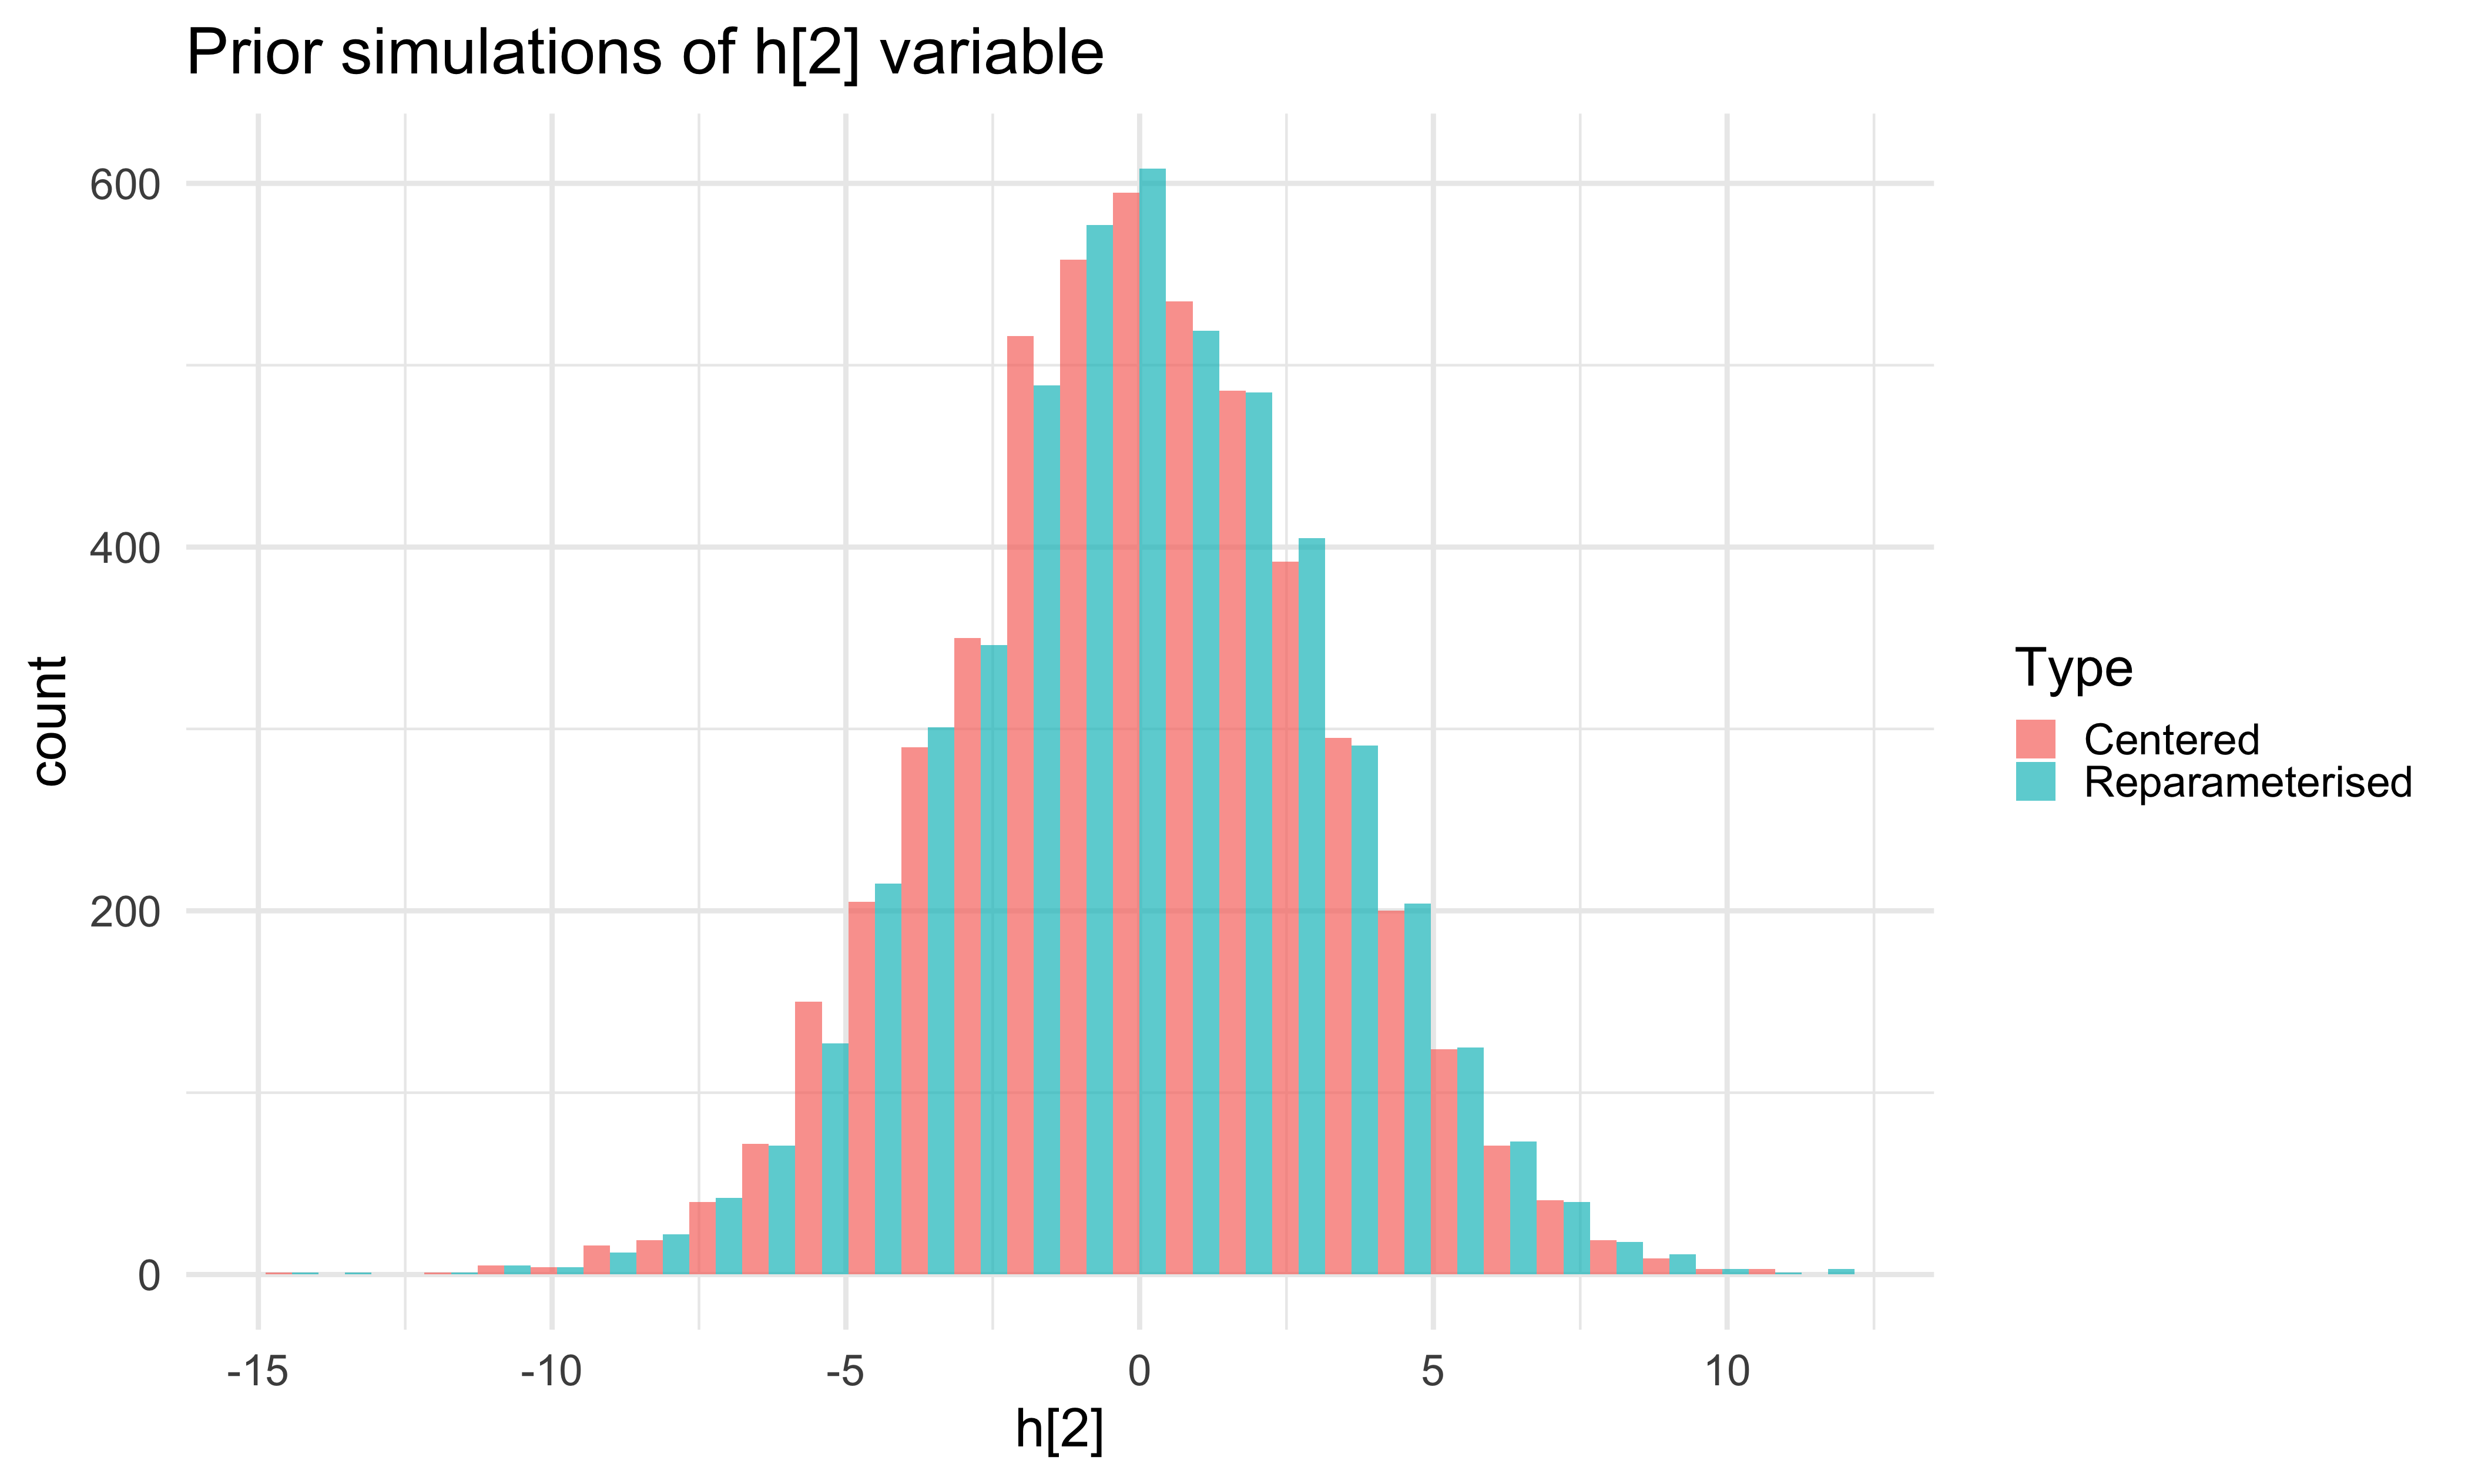
\includegraphics[scale=0.1]{figures/ppc_h2.png}
            \caption{Prior predictive samples of second state variable}
        \end{figure}
        
        % Emphasise here that different paramterisations of the models are the same model
        % Use a prior predictive check from both paramterisations show that the results are
        % the same


\section{Results}

    \subsection{Hamiltonian Monte Carlo}

    \subsection{Gaussian Mixture Approximation}

    \subsection{Reweigthing rank statistics of Gaussian Mixture}

\section{Discussion}

\subsection{Limitations}

\section{Conclusion}

\newpage

\bibliography{references}

\end{document}
